%Jennifer Pan, August 2011

\documentclass[10pt,letter]{article}
	% basic article document class
	% use percent signs to make comments to yourself -- they will not show up.

\usepackage{amsmath}
\usepackage{amssymb}
	% packages that allow mathematical formatting

\usepackage{graphicx}
	% package that allows you to include graphics

\usepackage{setspace}
	% package that allows you to change spacing

\onehalfspacing
	% text become 1.5 spaced

\usepackage{fullpage}
	% package that specifies normal margins

\renewcommand{\vector}[1]{\boldsymbol{#1}}
\newcommand{\problem}[1]{\section*{Problem #1}}
\newcommand{\problempart}[1]{\paragraph{#1}}

\begin{document}
	% line of code telling latex that your document is beginning


\title{ECON 511 Problem Set 1}

\author{Nicholas Wu}

\date{Spring 2021}
	% Note: when you omit this command, the current dateis automatically included

\maketitle
	% tells latex to follow your header (e.g., title, author) commands.
%\textbf{Note:} I use bold symbols to denote vectors and nonbolded symbols to denote scalars. I primarily use vector notation to shorthand some of the sums, since many of the sums are dot products.

\problem{1}
Code attached. I used Python (the Jupyter notebook is attached) and the pandas, numpy, and statsmodel (for HP filtering) packages.
\problem{2}
\problempart{(1)}
The FOC is
\[ w_t = \alpha K_t^{\alpha} (L^*_t)^{\alpha - 1} \]
\[ (L^*_t)^{1 - \alpha } = \frac{\alpha K_t^{\alpha}}{w_t} \]
\[ L^*_t = \left( \frac{\alpha K_t^{\alpha}}{w_t} \right)^{1/(1-\alpha)}\]
Plugging into the production function:
\[ Y_t = K_t^{\alpha} \left( \frac{\alpha K_t^{\alpha}}{w_t} \right)^{\alpha/(1-\alpha)} = \left( \frac{\alpha K_t}{w_t} \right)^{\alpha/(1-\alpha)} \]
So
\[ \pi(K_t, w_t) =  \left( \frac{\alpha K_t}{w_t} \right)^{\alpha/(1-\alpha)} - w_t\left( \frac{\alpha K_t^{\alpha}}{w_t} \right)^{1/(1-\alpha)} \]
\[ =  \left( \frac{\alpha K_t}{w_t} \right)^{\alpha/(1-\alpha)} - \left( \frac{\alpha K_t^{\alpha}}{w_t^\alpha} \right)^{1/(1-\alpha)} \]
\[ = (1 - \alpha)\left(\frac{\alpha K_t}{w_t} \right)^{\alpha/(1-\alpha)} \]
\problempart{(2)}
\[ V(K_t, w_t, p_t^K) = \max_{I_{t}}\left( \pi(K_t, w_t) - p_t^K I_{t} + \frac{1}{1+r}\mathbb{E}_t[V((1-\delta)K_t + I_t, (1+g)w_t, p^K_{t} \varepsilon_{t+1})] \right) \]
\problempart{(3)}
The FOCs are
\[ p_t^K = \frac{1}{1+r} \mathbb{E}_t[V_1((1-\delta)K_t + I_t, (1+g)w_t, p^K_{t} \varepsilon_{t+1})] \]
Applying the envelope theorem
\[ V_1(K_t, w_t, p_t^K) = \pi_1(K_t, w_t) + \frac{1-\delta}{1+r}\mathbb{E}_t[V_1((1-\delta)K_t + I_t, (1+g)w_t, p^K_{t} \varepsilon_{t+1})] \]
Taking expectations and using the law of iterated expectation to the first expression (at time $t+1$), we get
\[ \mathbb{E}_t p_{t+1}^K = \mathbb{E}_t \left(\frac{1}{1+r} V_1((1-\delta)K_{t+1} + I_{t+1}, (1+g)w_{t+1}, p^K_{t+1} \varepsilon_{t+2}) \right) \]
Plugging the envelope theorem in to the first expression and using the law of iterated expectation again
\[ p_t^K = \frac{1}{1+r} \mathbb{E}_t\left[\pi_1((1-\delta)K_{t}+I_t, (1+g)w_t) + \frac{1-\delta}{1+r}V_1((1-\delta)K_{t+1} + I_{t+1}, (1+g)w_{t+1}, p^K_{t+1} \varepsilon_{t+2})\right] \]
Simplifying out the terms equaling $\mathbb{E}_t p_{t+1}^K$, we get
\[ p_t^K = \frac{1}{1+r} \mathbb{E}_t\left[\pi_1((1-\delta)K_{t}+I_t, (1+g)w_t) + (1-\delta)p_{t+1}^K\right] \]
Since we determined $\pi$ in part 1,
\[ \pi_1((1-\delta)K_t + I_t, (1+g)w_t) = \alpha \left(\frac{\alpha}{(1+g)w_t} \right)^{\alpha/(1-\alpha)} K_{t+1}^{\alpha/(1-\alpha) - 1} \]
Plugging in
\[ (1+r)p_t^K = \mathbb{E}_t\left[\alpha \left(\frac{\alpha}{(1+g)w_t} \right)^{\alpha/(1-\alpha)} K_{t+1}^{\frac{2\alpha-1}{1-\alpha}} + (1-\delta)p_{t+1}^K\right] \]
\[ (1+r)p_t^K - (1-\delta)\mathbb{E}_tp_{t+1}^K = \alpha \left(\frac{\alpha}{(1+g)w_t} \right)^{\alpha/(1-\alpha)} K_{t+1}^{\frac{2\alpha-1}{1-\alpha}} \]
\[ \frac{p_t^K}{\alpha}\left(\frac{(1+g)w_t}{\alpha} \right)^{\alpha/(1-\alpha)}\left((1+r) - (1-\delta)\mathbb{E}_t\frac{p_{t+1}^K}{p_t^K}\right) =  K_{t+1}^{\frac{2\alpha-1}{1-\alpha}} \]
\[ K_{t+1}  = \left(\frac{p_t^K}{\alpha}\right)^{\frac{1-\alpha}{2\alpha-1}}\left(\frac{(1+g)w_t}{\alpha} \right)^{\frac{\alpha}{2\alpha - 1}}\left((1+r) - (1-\delta)\mathbb{E}_t\varepsilon_{t+1}\right)^{\frac{1-\alpha}{2\alpha-1}}   \]
\problempart{(4)}
Plugging in, we get
\[ K_{t+1}  = \left(\frac{p_t^K}{\alpha}\right)^{\frac{1-\alpha}{2\alpha-1}}\left(\frac{(1+g)w_t}{\alpha} \right)^{\frac{\alpha}{2\alpha - 1}}\left((1+r) - (1-\delta)e^{(1/2) \sigma^2 + \mu}\right)^{\frac{1-\alpha}{2\alpha-1}}   \]
\[ \ln K^*_{t+1} = \frac{1-\alpha}{2\alpha - 1} \left( \ln \left(\frac{p_t^K}{\alpha}\right) + \frac{\alpha}{1-\alpha} \ln \left(\frac{(1+g)w_t}{\alpha} \right) + \ln \left((1+r) - (1-\delta)e^{(1/2) \sigma^2 + \mu}\right)  \right) \]
\[ =  \frac{1-\alpha}{2\alpha - 1} \left( \ln p_t^K - \ln \alpha + \frac{\alpha}{1-\alpha} \left( \ln(1+g) + \ln w_t - \ln \alpha \right) + \ln(1+r) + \ln \left(1 - \frac{1-\delta}{1+r}e^{(1/2) \sigma^2 + \mu}\right)  \right) \]
\[ =  \frac{1-\alpha}{2\alpha - 1} \left( \ln p_t^K - \ln \alpha + \frac{\alpha}{1-\alpha} \left( \ln(1+g) + \ln w_t - \ln \alpha \right) + \ln(1+r) + \ln \left(1 - \frac{1-\delta}{1+r}e^{(1/2) \sigma^2 + \mu}\right)  \right) \]
\[ =  \frac{1-\alpha}{1 - 2\alpha} \left( - \ln p_t^K + \ln \alpha - \frac{\alpha}{1-\alpha} \left( \ln(1+g) + \ln w_t - \ln \alpha \right) - \ln(1+r) - \ln \left(1 - \frac{1-\delta}{1+r}e^{(1/2) \sigma^2 + \mu}\right)  \right) \]
\[ =  \frac{1-\alpha}{1 - 2\alpha} \left( \ln \alpha - \frac{\alpha}{1-\alpha} \left( \ln(1+g) + \ln w_t - \ln \alpha \right) - \ln(1+r)- \ln p_t^K - \ln \left(1 - \frac{1-\delta}{1+r}e^{(1/2) \sigma^2 + \mu}\right)  \right) \]
\[ =  \frac{1-\alpha}{1 - 2\alpha} \left( \frac{1}{1-\alpha} \left( (1-\alpha)\ln \alpha - \alpha \ln(1+g) - \alpha \ln w_t + \alpha \ln \alpha \right) - \ln(1+r)- \ln p_t^K - \ln \left(1 - \frac{1-\delta}{1+r}e^{(1/2 )\sigma^2 + \mu}\right)  \right) \]
\[ =  \frac{1-\alpha}{1 - 2\alpha} \left( \frac{1}{1-\alpha} \left( \ln \alpha - \alpha (\ln(1+g) + \ln w_t)  \right) - \ln(1+r)- \ln p_t^K - \ln \left(1 - \frac{1-\delta}{1+r}e^{(1/2) \sigma^2 + \mu}\right)  \right) \]
which is the desired expression. $K_t$ does not play a role since there are no adjustment costs, and so the decision on how much capital to invest tomorrow is only based on the prices today rather than the capital stock today.
\problempart{(5)}
Since
\[ K_{t+1} = (1-\delta)K_t + I_t \]
\[ K_{t+1} / K_t = 1 - \delta + I_t/K_t = 1 + i_t \]
\[ i_t \approx \ln(1+i_t) = \ln K_{t+1} - \ln K_t \]
\[ = \frac{1-\alpha}{1 - 2\alpha} \left( \frac{1}{1-\alpha} \left( - \alpha ( \ln w_t - \ln w_{t-1})  \right) - \ln p_t^K + \ln p_{t-1}^K  \right) \]
\[ = \frac{1-\alpha}{1 - 2\alpha} \left( \frac{1}{1-\alpha} \left( - \alpha ( \ln (1+g))  \right) - \ln \varepsilon_t  \right) \]
\[ =  -\frac{\alpha}{1 - 2\alpha} \ln (1+g) - \frac{1-\alpha}{1 - 2\alpha}  \ln \varepsilon_t  \]
\[ \approx -\frac{\alpha}{1 - 2\alpha} g - \frac{1-\alpha}{1 - 2\alpha}  \ln \varepsilon_t \]
Investment ratio is decreasing in $g$ growth rate of wages and $\varepsilon_t$ the ratio increase in capital prices.
\problempart{(6)}
Since $\varepsilon_t$ are all independent, $corr(i_t, i_{t-1}) = 0$. Since $\ln \varepsilon_t$ is normal, we have that $i_t$ is also normal (affine function of a normal random variable is normal) so
\[ \mathbb{E}i_t = -\frac{\alpha}{1 - 2\alpha} g - \frac{1-\alpha}{1 - 2\alpha}\mu  \]
\[ V(i_t) = \left(\frac{1-\alpha}{1 - 2\alpha}\right)^2 \sigma^2  \]
Investment is determined by the current shock.
\problempart{(7)}
It is independent of $r$, since changes in $r$ proportionally impact both $K_t$ and $K_{t+1}$ and the effect cancels out. The investment rate is decreasing in $g$; if it is going to get more expensive to hire labor to optimally use capital, firms will invest less.
\problem{3}
\problempart{(1)}
From Question 2 part 3, we have
\[ K_{t+1}  = \left(\frac{p_t^K}{\alpha}\right)^{\frac{1-\alpha}{2\alpha-1}}\left(\frac{(1+g)w_t}{\alpha} \right)^{\frac{\alpha}{2\alpha - 1}}\left((1+r) - (1-\delta)\mathbb{E}_t \frac{p_{t+1}^K}{p_t^K} \right)^{\frac{1-\alpha}{2\alpha-1}}   \]
Since
\[ \mathbb{E}\frac{p_{t+1}^K}{p_t^K} = \frac{1}{(p_t^{K})^{0.05}}\mathbb{E}\varepsilon_{t+1} \]
We get
\[ K_{t+1}  = \left(\frac{p_t^K}{\alpha}\right)^{\frac{1-\alpha}{2\alpha-1}}\left(\frac{(1+g)w_t}{\alpha} \right)^{\frac{\alpha}{2\alpha - 1}}\left((1+r) - \frac{1-\delta}{(p_t^{K})^{0.05}}\mathbb{E}_t\varepsilon_{t+1}\right)^{\frac{1-\alpha}{2\alpha-1}}   \]
\[ = \left(\frac{p_t^K}{\alpha}\right)^{\frac{1-\alpha}{2\alpha-1}}\left(\frac{(1+g)w_t}{\alpha} \right)^{\frac{\alpha}{2\alpha - 1}}\left((1+r) - \frac{1-\delta}{(p_t^{K})^{0.05}} e^{(\sigma^2)/2 + \mu}\right)^{\frac{1-\alpha}{2\alpha-1}} \]

\problempart{(2)}
The policy function numerically computed is graphed.

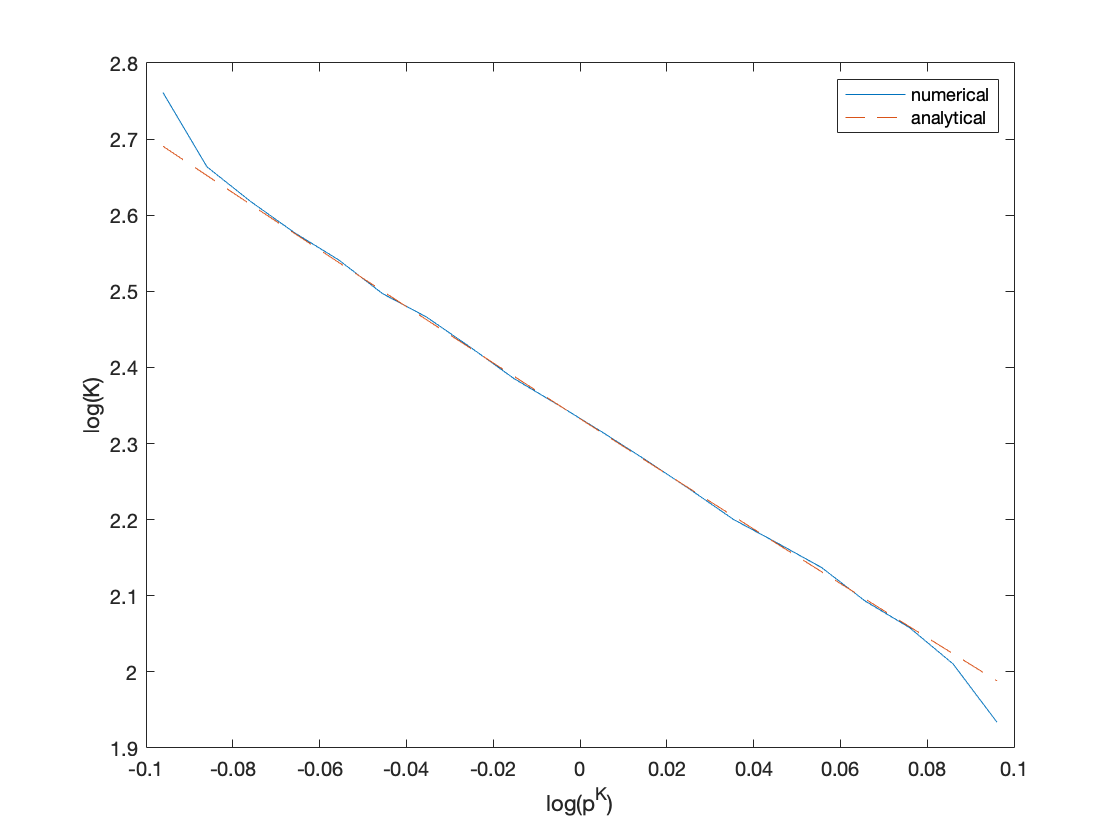
\includegraphics[width=15cm]{ps1fig1}

We verify that $r$ does impact investment rate this time. Because of the mean reversion in the prices, we can say that the firms can benefit by being more patient this time and wait through periods of higher prices. In the random walk case, there is no inherent mean reversion, and so $r$ does not impact $i$.
\problempart{(3)} The policy function computed under deterministic price reversion is below

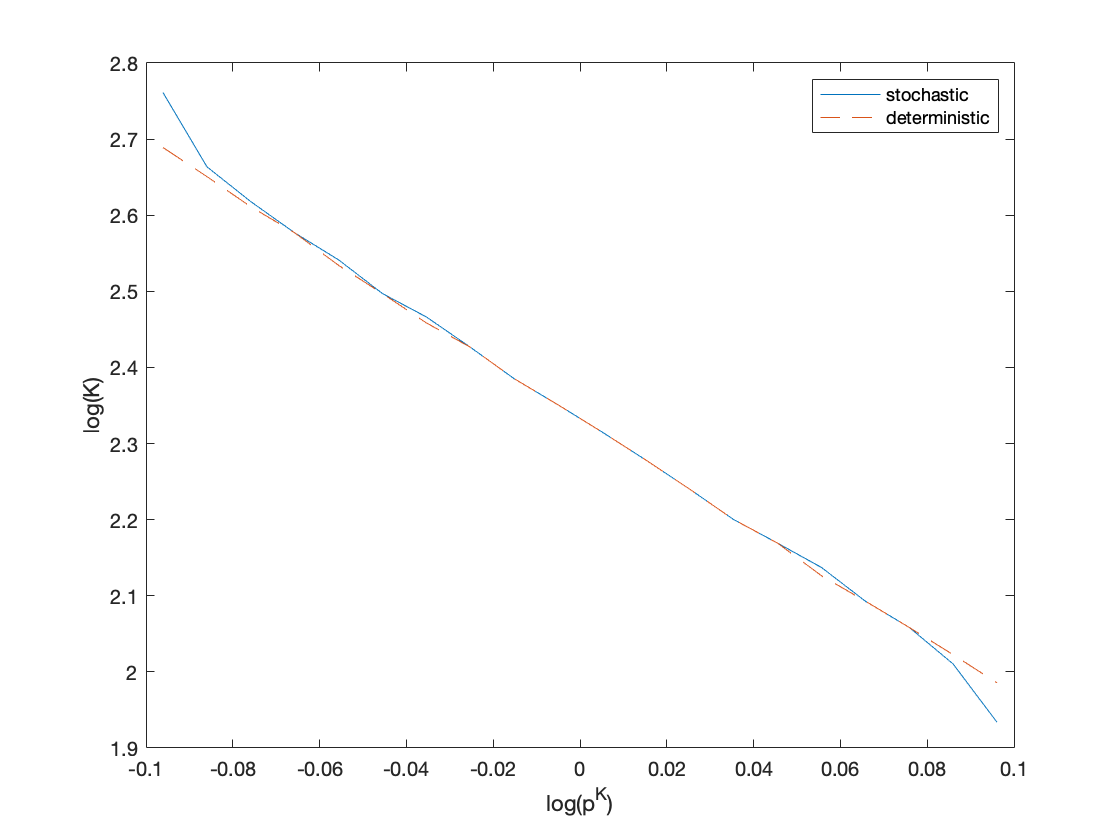
\includegraphics[width=15cm]{ps1fig2}

We see that investment is slightly higher when price is stochastic. This is because agents have the knowledge that the price is mean reverting, and can be patient and wait for prices to revert if the prices are high. However, under the stochastic setting, there is potential that the price process stays arbitrarily high forever, and hence the period investment is higher.
\end{document}
	% line of code telling latex that your document is ending. If you leave this out, you'll get an error
